\begin{frame}{El déficit total del GNC fue 6,4\% del PIB en 2025}
\centering
\resizebox{0.88\textwidth}{!}{
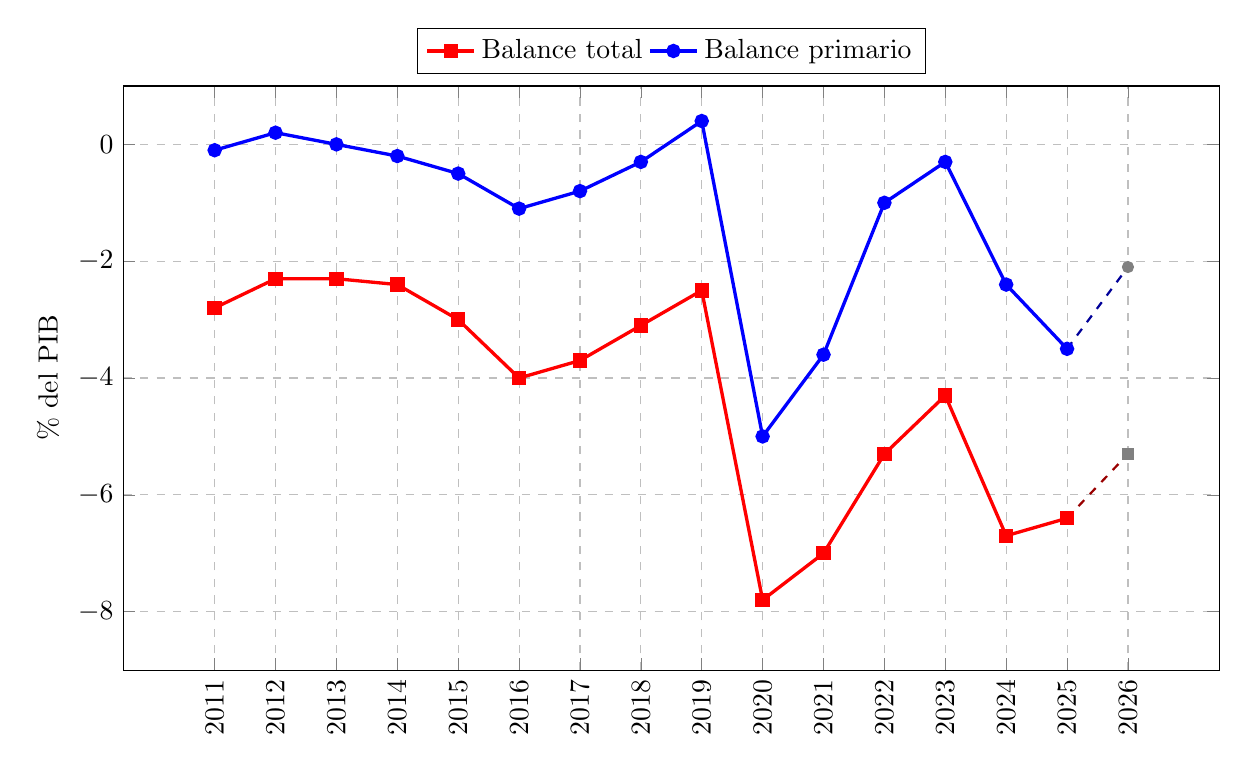
\begin{tikzpicture}
\begin{axis}[
    width=15.5cm,
    height=9cm,
    ylabel={\% del PIB},
    xtick={7,8,...,22},
    xticklabels={2011,2012,2013,2014,2015,2016,2017,2018,2019,2020,2021,2022,2023,2024,2025,2026},
    x tick label style={rotate=90,anchor=east},
    ymin=-9,
    ymax=1,
    grid=both,
    grid style=dashed,
    legend style={at={(0.5,1.02)},anchor=south,legend columns=-1}
]
\addplot[color=red,mark=square*,very thick] coordinates {
    (7,-2.8) (8,-2.3) (9,-2.3) (10,-2.4) (11,-3.0) (12,-4.0)
    (13,-3.7) (14,-3.1) (15,-2.5) (16,-7.8) (17,-7.0) (18,-5.3)
    (19,-4.3) (20,-6.7) (21,-6.4)
};
\addlegendentry{Balance total}
\addplot[color=blue,mark=*,very thick] coordinates {
    (7,-0.1) (8,0.2) (9,0.0) (10,-0.2) (11,-0.5) (12,-1.1)
    (13,-0.8) (14,-0.3) (15,0.4) (16,-5.0) (17,-3.6) (18,-1.0)
    (19,-0.3) (20,-2.4) (21,-3.5)
};
\addlegendentry{Balance primario}
\addplot[color=red!60!black,dashed,thick] coordinates {(21,-6.4) (22,-5.3)};
\addplot[color=blue!60!black,dashed,thick] coordinates {(21,-3.5) (22,-2.1)};
\addplot[color=gray,mark=square*,only marks] coordinates {(22,-5.3)};
\addplot[color=gray,mark=*,only marks] coordinates {(22,-2.1)};
\end{axis}
\end{tikzpicture}}
\scriptsize Línea sólida: resultados observados hasta 2025. Línea discontinua: proyección 2026.
\note{[Sources] MFMP 2026, capítulo 1, tabla 1.3. Serie histórica previa: MHCP, como en la versión fuente.}
\end{frame}